% Created by tikzDevice version 0.10.1 on 2016-04-22 17:26:01
% !TEX encoding = UTF-8 Unicode
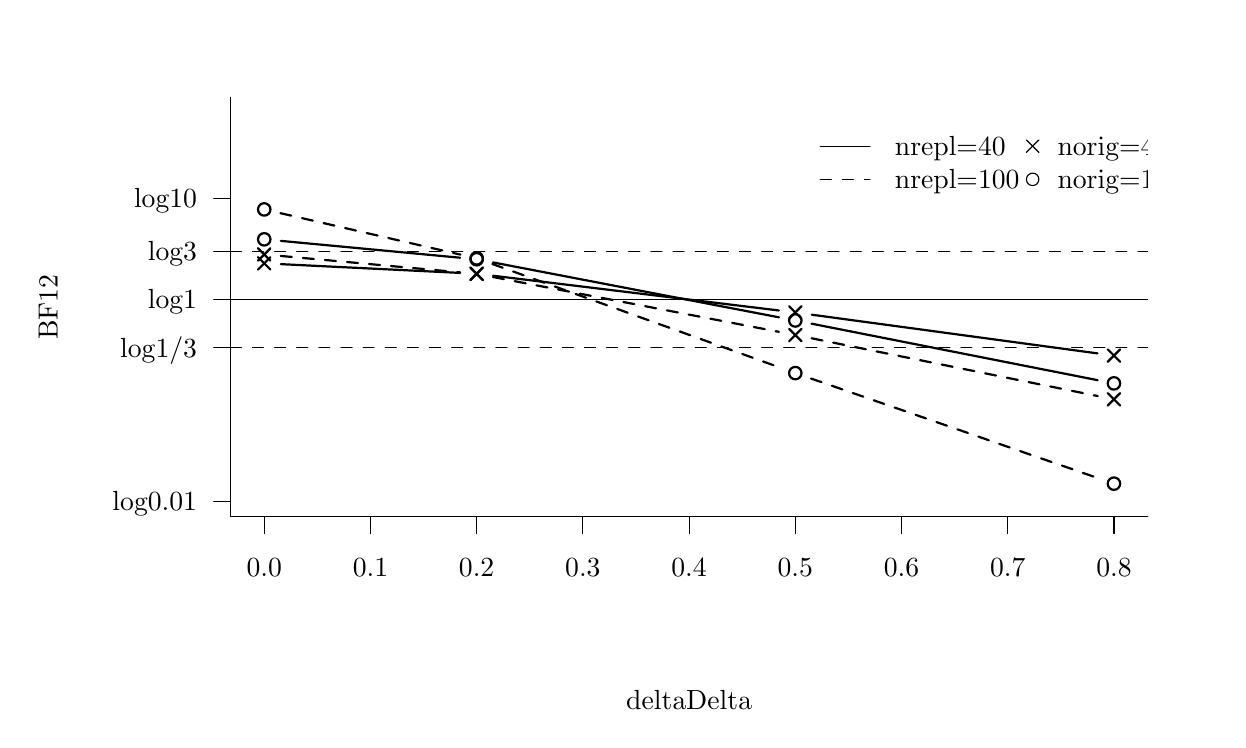
\begin{tikzpicture}[x=1pt,y=1pt]
\definecolor{fillColor}{RGB}{255,255,255}
\path[use as bounding box,fill=fillColor,fill opacity=0.00] (0,0) rectangle (430.00,250.00);
\begin{scope}
\path[clip] ( 73.20, 73.20) rectangle (404.80,224.80);
\definecolor{drawColor}{RGB}{0,0,0}

\path[draw=drawColor,line width= 0.8pt,line join=round,line cap=round] ( 91.47,164.55) -- (156.25,161.38);

\path[draw=drawColor,line width= 0.8pt,line join=round,line cap=round] (168.20,160.36) -- (271.42,147.81);

\path[draw=drawColor,line width= 0.8pt,line join=round,line cap=round] (283.33,146.28) -- (386.57,132.30);

\path[draw=drawColor,line width= 0.8pt,line join=round,line cap=round] ( 83.23,162.59) -- ( 87.73,167.09);

\path[draw=drawColor,line width= 0.8pt,line join=round,line cap=round] ( 83.23,167.09) -- ( 87.73,162.59);

\path[draw=drawColor,line width= 0.8pt,line join=round,line cap=round] (159.99,158.83) -- (164.49,163.33);

\path[draw=drawColor,line width= 0.8pt,line join=round,line cap=round] (159.99,163.33) -- (164.49,158.83);

\path[draw=drawColor,line width= 0.8pt,line join=round,line cap=round] (275.13,144.83) -- (279.63,149.33);

\path[draw=drawColor,line width= 0.8pt,line join=round,line cap=round] (275.13,149.33) -- (279.63,144.83);

\path[draw=drawColor,line width= 0.8pt,line join=round,line cap=round] (390.27,129.25) -- (394.77,133.75);

\path[draw=drawColor,line width= 0.8pt,line join=round,line cap=round] (390.27,133.75) -- (394.77,129.25);
\end{scope}
\begin{scope}
\path[clip] (  0.00,  0.00) rectangle (430.00,250.00);
\definecolor{drawColor}{RGB}{0,0,0}

\path[draw=drawColor,line width= 0.4pt,line join=round,line cap=round] ( 73.20,224.80) --
	( 73.20, 73.20) --
	(404.80, 73.20);
\end{scope}
\begin{scope}
\path[clip] (  0.00,  0.00) rectangle (430.00,250.00);
\definecolor{drawColor}{RGB}{0,0,0}

\node[text=drawColor,anchor=base,inner sep=0pt, outer sep=0pt, scale=  1.00] at (239.00,  3.60) {deltaDelta};

\node[text=drawColor,rotate= 90.00,anchor=base,inner sep=0pt, outer sep=0pt, scale=  1.00] at ( 10.80,149.00) {BF12};
\end{scope}
\begin{scope}
\path[clip] ( 73.20, 73.20) rectangle (404.80,224.80);
\definecolor{drawColor}{RGB}{0,0,0}

\path[draw=drawColor,line width= 0.8pt,dash pattern=on 4pt off 4pt ,line join=round,line cap=round] ( 91.46,167.51) -- (156.27,161.58);

\path[draw=drawColor,line width= 0.8pt,dash pattern=on 4pt off 4pt ,line join=round,line cap=round] (168.13,159.90) -- (271.49,140.08);

\path[draw=drawColor,line width= 0.8pt,dash pattern=on 4pt off 4pt ,line join=round,line cap=round] (283.26,137.76) -- (386.64,116.89);

\path[draw=drawColor,line width= 0.8pt,line join=round,line cap=round] ( 83.23,165.80) -- ( 87.73,170.30);

\path[draw=drawColor,line width= 0.8pt,line join=round,line cap=round] ( 83.23,170.30) -- ( 87.73,165.80);

\path[draw=drawColor,line width= 0.8pt,line join=round,line cap=round] (159.99,158.79) -- (164.49,163.29);

\path[draw=drawColor,line width= 0.8pt,line join=round,line cap=round] (159.99,163.29) -- (164.49,158.79);

\path[draw=drawColor,line width= 0.8pt,line join=round,line cap=round] (275.13,136.69) -- (279.63,141.19);

\path[draw=drawColor,line width= 0.8pt,line join=round,line cap=round] (275.13,141.19) -- (279.63,136.69);

\path[draw=drawColor,line width= 0.8pt,line join=round,line cap=round] (390.27,113.45) -- (394.77,117.95);

\path[draw=drawColor,line width= 0.8pt,line join=round,line cap=round] (390.27,117.95) -- (394.77,113.45);

\path[draw=drawColor,line width= 0.8pt,line join=round,line cap=round] ( 91.46,172.96) -- (156.27,166.87);

\path[draw=drawColor,line width= 0.8pt,line join=round,line cap=round] (168.13,165.18) -- (271.49,145.33);

\path[draw=drawColor,line width= 0.8pt,line join=round,line cap=round] (283.27,143.03) -- (386.63,122.62);

\path[draw=drawColor,line width= 0.8pt,line join=round,line cap=round] ( 85.48,173.52) circle (  2.25);

\path[draw=drawColor,line width= 0.8pt,line join=round,line cap=round] (162.24,166.31) circle (  2.25);

\path[draw=drawColor,line width= 0.8pt,line join=round,line cap=round] (277.38,144.20) circle (  2.25);

\path[draw=drawColor,line width= 0.8pt,line join=round,line cap=round] (392.52,121.46) circle (  2.25);

\path[draw=drawColor,line width= 0.8pt,dash pattern=on 4pt off 4pt ,line join=round,line cap=round] ( 91.33,182.97) -- (156.39,167.99);

\path[draw=drawColor,line width= 0.8pt,dash pattern=on 4pt off 4pt ,line join=round,line cap=round] (167.89,164.61) -- (271.73,127.22);

\path[draw=drawColor,line width= 0.8pt,dash pattern=on 4pt off 4pt ,line join=round,line cap=round] (283.05,123.22) -- (386.85, 87.20);

\path[draw=drawColor,line width= 0.8pt,line join=round,line cap=round] ( 85.48,184.32) circle (  2.25);

\path[draw=drawColor,line width= 0.8pt,line join=round,line cap=round] (162.24,166.64) circle (  2.25);

\path[draw=drawColor,line width= 0.8pt,line join=round,line cap=round] (277.38,125.18) circle (  2.25);

\path[draw=drawColor,line width= 0.8pt,line join=round,line cap=round] (392.52, 85.23) circle (  2.25);

\path[] (277.38,219.19) rectangle (362.90,183.19);

\path[draw=drawColor,line width= 0.4pt,line join=round,line cap=round] (286.38,207.19) -- (304.38,207.19);

\path[draw=drawColor,line width= 0.4pt,dash pattern=on 4pt off 4pt ,line join=round,line cap=round] (286.38,195.19) -- (304.38,195.19);

\node[text=drawColor,anchor=base west,inner sep=0pt, outer sep=0pt, scale=  1.00] at (313.38,203.74) {nrepl=40};

\node[text=drawColor,anchor=base west,inner sep=0pt, outer sep=0pt, scale=  1.00] at (313.38,191.74) {nrepl=100};

\path[] (354.14,219.19) rectangle (421.66,183.19);

\path[draw=drawColor,line width= 0.4pt,line join=round,line cap=round] (360.89,204.94) -- (365.39,209.44);

\path[draw=drawColor,line width= 0.4pt,line join=round,line cap=round] (360.89,209.44) -- (365.39,204.94);

\path[draw=drawColor,line width= 0.4pt,line join=round,line cap=round] (363.14,195.19) circle (  2.25);

\node[text=drawColor,anchor=base west,inner sep=0pt, outer sep=0pt, scale=  1.00] at (372.14,203.74) {norig=40};

\node[text=drawColor,anchor=base west,inner sep=0pt, outer sep=0pt, scale=  1.00] at (372.14,191.74) {norig=100};
\end{scope}
\begin{scope}
\path[clip] (  0.00,  0.00) rectangle (430.00,250.00);
\definecolor{drawColor}{RGB}{0,0,0}

\path[draw=drawColor,line width= 0.4pt,line join=round,line cap=round] ( 85.48, 73.20) -- (392.52, 73.20);

\path[draw=drawColor,line width= 0.4pt,line join=round,line cap=round] ( 85.48, 73.20) -- ( 85.48, 67.20);

\path[draw=drawColor,line width= 0.4pt,line join=round,line cap=round] (123.86, 73.20) -- (123.86, 67.20);

\path[draw=drawColor,line width= 0.4pt,line join=round,line cap=round] (162.24, 73.20) -- (162.24, 67.20);

\path[draw=drawColor,line width= 0.4pt,line join=round,line cap=round] (200.62, 73.20) -- (200.62, 67.20);

\path[draw=drawColor,line width= 0.4pt,line join=round,line cap=round] (239.00, 73.20) -- (239.00, 67.20);

\path[draw=drawColor,line width= 0.4pt,line join=round,line cap=round] (277.38, 73.20) -- (277.38, 67.20);

\path[draw=drawColor,line width= 0.4pt,line join=round,line cap=round] (315.76, 73.20) -- (315.76, 67.20);

\path[draw=drawColor,line width= 0.4pt,line join=round,line cap=round] (354.14, 73.20) -- (354.14, 67.20);

\path[draw=drawColor,line width= 0.4pt,line join=round,line cap=round] (392.52, 73.20) -- (392.52, 67.20);

\node[text=drawColor,anchor=base,inner sep=0pt, outer sep=0pt, scale=  1.00] at ( 85.48, 51.60) {0.0};

\node[text=drawColor,anchor=base,inner sep=0pt, outer sep=0pt, scale=  1.00] at (123.86, 51.60) {0.1};

\node[text=drawColor,anchor=base,inner sep=0pt, outer sep=0pt, scale=  1.00] at (162.24, 51.60) {0.2};

\node[text=drawColor,anchor=base,inner sep=0pt, outer sep=0pt, scale=  1.00] at (200.62, 51.60) {0.3};

\node[text=drawColor,anchor=base,inner sep=0pt, outer sep=0pt, scale=  1.00] at (239.00, 51.60) {0.4};

\node[text=drawColor,anchor=base,inner sep=0pt, outer sep=0pt, scale=  1.00] at (277.38, 51.60) {0.5};

\node[text=drawColor,anchor=base,inner sep=0pt, outer sep=0pt, scale=  1.00] at (315.76, 51.60) {0.6};

\node[text=drawColor,anchor=base,inner sep=0pt, outer sep=0pt, scale=  1.00] at (354.14, 51.60) {0.7};

\node[text=drawColor,anchor=base,inner sep=0pt, outer sep=0pt, scale=  1.00] at (392.52, 51.60) {0.8};

\path[draw=drawColor,line width= 0.4pt,line join=round,line cap=round] ( 73.20, 78.81) -- ( 73.20,188.33);

\path[draw=drawColor,line width= 0.4pt,line join=round,line cap=round] ( 73.20, 78.81) -- ( 67.20, 78.81);

\path[draw=drawColor,line width= 0.4pt,line join=round,line cap=round] ( 73.20,134.41) -- ( 67.20,134.41);

\path[draw=drawColor,line width= 0.4pt,line join=round,line cap=round] ( 73.20,151.83) -- ( 67.20,151.83);

\path[draw=drawColor,line width= 0.4pt,line join=round,line cap=round] ( 73.20,169.25) -- ( 67.20,169.25);

\path[draw=drawColor,line width= 0.4pt,line join=round,line cap=round] ( 73.20,188.33) -- ( 67.20,188.33);

\node[text=drawColor,anchor=base east,inner sep=0pt, outer sep=0pt, scale=  1.00] at ( 61.20, 75.37) {log0.01};

\node[text=drawColor,anchor=base east,inner sep=0pt, outer sep=0pt, scale=  1.00] at ( 61.20,130.97) {log1/3};

\node[text=drawColor,anchor=base east,inner sep=0pt, outer sep=0pt, scale=  1.00] at ( 61.20,148.38) {log1};

\node[text=drawColor,anchor=base east,inner sep=0pt, outer sep=0pt, scale=  1.00] at ( 61.20,165.80) {log3};

\node[text=drawColor,anchor=base east,inner sep=0pt, outer sep=0pt, scale=  1.00] at ( 61.20,184.89) {log10};
\end{scope}
\begin{scope}
\path[clip] ( 73.20, 73.20) rectangle (404.80,224.80);
\definecolor{drawColor}{RGB}{0,0,0}

\path[draw=drawColor,line width= 0.4pt,line join=round,line cap=round] ( 73.20,151.83) -- (404.80,151.83);

\path[draw=drawColor,line width= 0.4pt,dash pattern=on 4pt off 4pt ,line join=round,line cap=round] ( 73.20,134.41) -- (404.80,134.41);

\path[draw=drawColor,line width= 0.4pt,dash pattern=on 4pt off 4pt ,line join=round,line cap=round] ( 73.20,169.25) -- (404.80,169.25);
\end{scope}
\end{tikzpicture}
